\section{Théorie}
\subsection{Video Graphics Array (VGA)}
Le VGA (Video Graphics Array) est un standard qui à l'origine a été développé pour l'affichage sur des écrans CRT (Cathode Ray Tube). Un écran à tube cathodique contient un canon à électrons dont le rayon balaye l'écran phosphorescent et produit de la lumière au contact de ce dernier. Le mouvement de balayage est réalisé grâce à des bobines produisant des champs magnétiques dans le tube, une paire de bobines permet le balayage horizontal et l'autre paire permet le balayage vertical. Dans le cas d'un tube couleur, celui-ci possède trois canons à électrons dont les rayons vont passer par un masque (Shadow mask ou masque utilisé sur tube Trinitron) afin d'afficher la couleur souhaitée.\\

Le standard VGA est également disponible sur les écrans LCD, et bien que la technologie soit différente, le comportement d'un écran CRT est reproduit. Le principe d'affichage reste donc le même dans les deux cas.\\

\begin{figure}[h!]
	\centering
	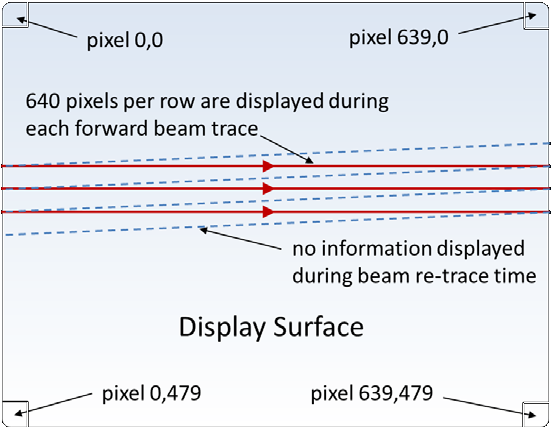
\includegraphics[scale=0.6]{images/scan.png}
	\caption{Balayage de l'écran \cite{cite:scan}}
	\label{fig:scan}
\end{figure}

L'écran est balayé de gauche à droite et de bas en haut, afin d'afficher une couleur pixel par pixel. Une fois le rayon arrivé en fin d'une ligne ou en bas à droite de l'écran, des temps d'attentes sont introduits, en effet dans le cas d'un tube cathodique cela s'expliquait par le temps nécessaire au tube pour revenir en début de ligne ou début d'écran (pixel en haut à gauche).\\

\begin{figure}[h!]
	\centering
	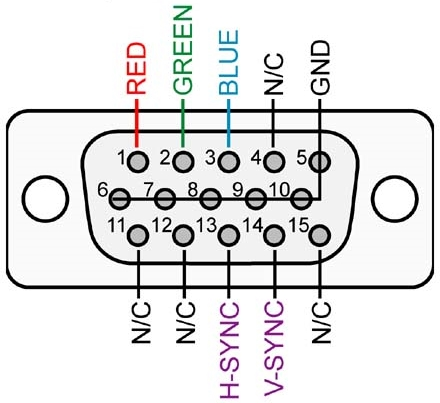
\includegraphics[scale=1.0]{images/vgapinout.jpg}
	\caption{Connecteur VGA mâle \cite{cite:vgapinout}}
	\label{fig:vgapinout}
\end{figure}

\newpage
Le connecteur VGA possède 15 pins (connecteur D-SUB 15-pin), 3 pins sont utilisés pour les signaux de couleurs (rouge, vert et bleu), 1 pin est utilisé pour la masse et 2 pins correspondent aux signaux de synchronisation \emph{hsync} et \emph{vsync}.\\

Parmi les signaux à produire listés ci-dessus, des signaux correspondent aux couleurs primaires rouge, vert et bleu. Ces signaux possèdent une tension comprise entre 0 et 0.7 volts et permettent, pour un pixel donné de déterminer sa couleur finale. Une couleur est une information qui peut être codée sous forme de signal numérique sur plusieurs bits.

\begin{snugshade}
\noindent \textbf{Exemple}: si le rouge est codé sur 3 bits, le vert sur 3 bits, et le vert sur 2 bits, il y aura alors $2^8 = 256$ possibilités de couleurs pour un pixel donné.
\end{snugshade}

\noindent Cette information numérique nécessite d'être convertie en signal analogique afin de pouvoir être exploitée par l'écran. En effet, les signaux de couleurs possèdent une tension que nous souhaitons faire varier afin de modifier l'intensité des couleurs. Pour convertir une information numérique en signal analogique, nous avons besoin d'un convertisseur numérique analogique (DAC). Ci-dessous le schéma d'un DAC 3 bits pour la couleur rouge et le calcul associé donnant la tension de sortie avec ce choix de résistances pour les 3 entrées à l'état haut.\\

\begin{multicols}{2}
	\noindent
	\begin{minipage}{\linewidth}
		\centering
		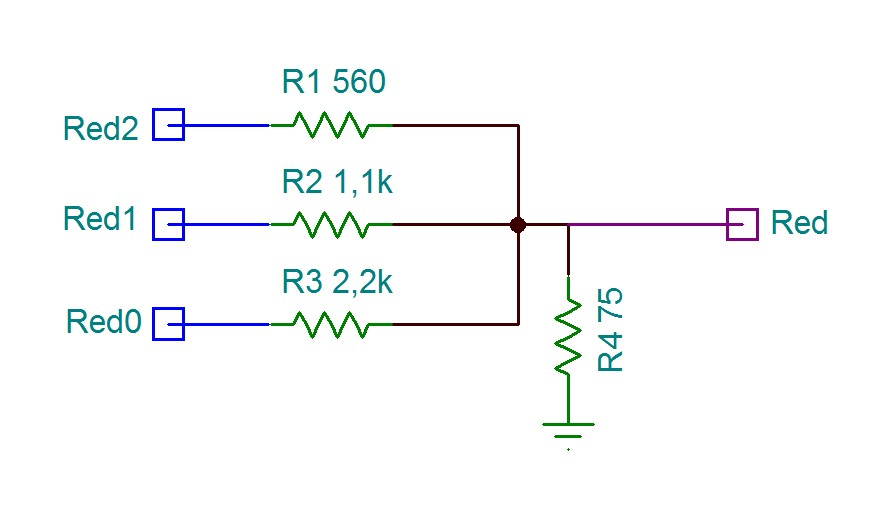
\includegraphics[scale = 0.25]{images/simple_dac.jpg}
		\captionof{figure}{VGA timing \cite{cite:psocvga}}
		\label{fig:vgadac}
	\end{minipage}
	
	\begin{flalign*}
	V_{red} = &\frac{\frac{3.3}{560} + \frac{3.3}{1100} + \frac{3.3}{2200}}{\frac{1}{560} + \frac{1}{1100} + \frac{1}{2200} + \frac{1}{75}}&\\
			= &0.63 V&
	\end{flalign*}
\end{multicols}

Les signaux \emph{hsync} et \emph{vsync} sont respectivement les signaux de synchronisation horizontale et verticale. Ce sont tous deux des signaux actifs à l'état bas. Le signal \emph{hsync} devient actif lorsqu'une ligne a été parcourue et que le canon à électrons doit se repositionner au début de la ligne suivante. Le signal \emph{vsync} devient actif lorsque le dernier pixel a été atteint en bas à droite de l'écran et que le canon à électrons doit se repositionner au début de l'écran (en haut à gauche). Les deux signaux de synchronisation sont actifs pendant une durée \emph{sync pulse} qui elle même est entourée par une durée \emph{back porch} et une durée \emph{front porch}. Ces durées sont différentes pour le parcours horizontal et vertical de l'écran, et dépendent également de la résolution choisie ainsi que la fréquence de rafraîchissement de l'écran. De plus, la fréquence à laquelle l'écran doit être parcouru dépend également de ces informations.
\begin{snugshade}
\noindent \textbf{VGA 640 x 480 60 Hz \cite{cite:timingsvga}}
\begin{center}
	Général\\
	\begin{tabular}{| l | l |}
	\hline
	Fréquence de rafraîchissement & 60 Hz\\ \hline
	Fréquence balayage pixels & 25.175 MHz\\ \hline
	\end{tabular}
\end{center}

\begin{center}
	Horizontal\\
	\begin{tabular}{| l | l |}
	\hline
	Zone visible & 640 px\\ \hline
	Front porch & 16 px\\ \hline
	Sync pulse & 96 px\\ \hline
	Back porch & 48 px\\ \hline
	\end{tabular}
\end{center}

\begin{center}
	Vertical\\
	\begin{tabular}{| l | l |}
	\hline
	Zone visible & 480 px\\ \hline
	Front porch & 10 px\\ \hline
	Sync pulse & 2 px\\ \hline
	Back porch & 33 px\\ \hline
	\end{tabular}
\end{center}

\end{snugshade}

\begin{figure}[h!]
	\centering
	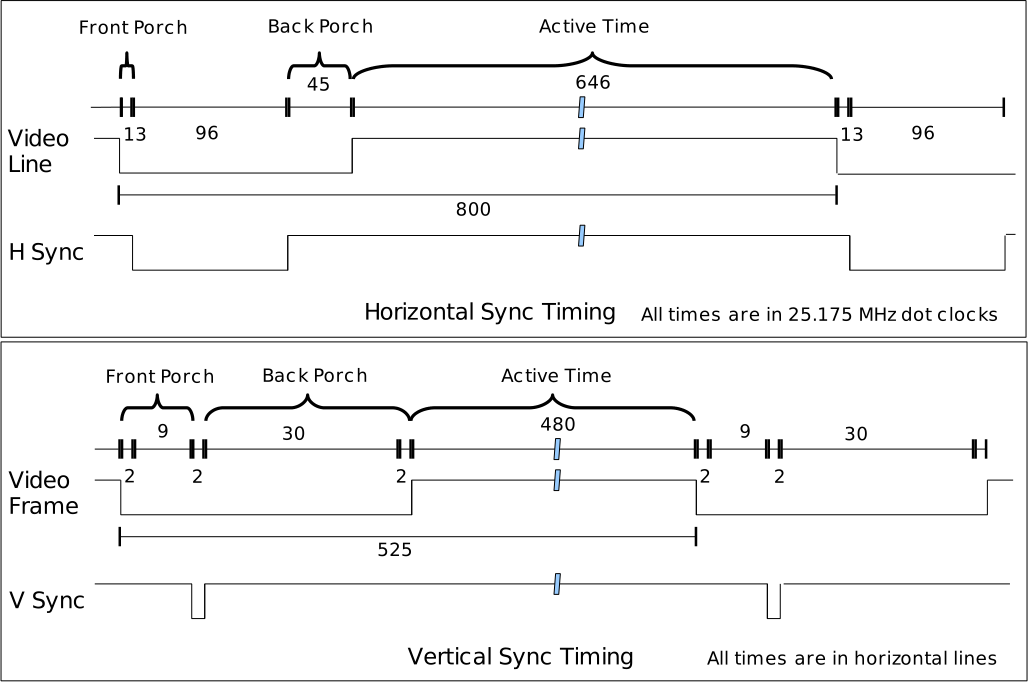
\includegraphics[scale=0.45]{images/vgatiming.png}
	\caption{Timings VGA \cite{cite:psocvga}}
	\label{fig:vgatiming}
\end{figure}

\noindent \textbf{N.B.} Les timings du tableau \cite{cite:timingsvga} et du schéma \cite{cite:psocvga} sont différents, ceux que nous avons choisis sont ceux du tableau.

\newpage
\subsection{Protocole PS/2 clavier}
Utilisant la DE0-Nano, nous souhaitions pouvoir avoir accès à des boutons supplémentaires et plus accessibles que sur la carte. Nous avons donc opté pour l'utilisation d'un clavier.\\

\begin{figure}[h!]
	\centering
	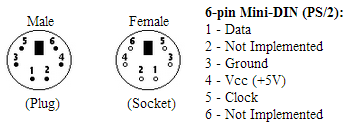
\includegraphics{images/ps2.png}
	\caption{6-pin Mini-DIN (PS/2) \cite{cite:ps2protocol}}
	\label{fig:ps2}
\end{figure}

Le connecteur PS/2 utilisé est un port mini-DIN possédant 6 broches (figure \ref{fig:ps2}). Celles qui nous intéressent sont la \emph{masse}, \emph{VCC (5V)}, \emph{Clock} et \emph{Data}. La ligne de données, \emph{Data}, est bidirectionnelle : le clavier peut communiquer avec le matériel connecté (envoie de données concernant les touches enfoncées) et inversement, nous n'utiliserons cependant que la communication clavier vers FPGA.\\

L'état par défaut des lignes \emph{Data} et \emph{Clock,} l'état d'attente, correspond à un 1 logique. Pour indiquer qu'une donnée est prête à être récupérée sur le signal \emph{Data}, le clavier met le signal \emph{Clock} à l'état bas. Les 8 bits de données peuvent ensuite être lus en série sur \emph{Data} sachant que le bit de poids faible sera envoyé en premier. Un bit de parité est ensuite envoyé, celui-ci permet la détection d'erreurs. Enfin, un bit de stop est envoyé pour indiquer la fin de la communication. Ci-dessous un récapitulatif des étapes de la communication clavier vers matériel.

\begin{enumerate}
\item 1 bit de \textbf{départ} : 0
\item 8 bits de \textbf{données}
\item 1 bit de \textbf{parité}
\item 1 bit de \textbf{fin} : 1\\
\end{enumerate}

% TODO parler du bit de parité

Le clavier envoie des \textbf{Scan codes}, ceux-ci permettent de représenter les différentes touches du clavier. Il existe deux types de codes: le premier type sert lors de l'appui sur une touche (make code), tandis que le second représente le relâchement d'une touche (break code). Un code peut comporter plusieurs octets, c'est le cas de la plupart des break codes. Le tableau suivant a été utilisé afin d'avoir la correspondance de chaque touche à ses codes: \href{http://www.computer-engineering.org/ps2keyboard/scancodes2.html}{http://www.computer-engineering.org/ps2keyboard/scancodes2.html}.\\
\textbf{N.B.} La correspondance entre touche et codes du tableau ci-dessus concerne les claviers QWERTY.\\

\newpage
